\chapter{Evaluation}

\section{Technical Evaluation}
%Voxelizer, polygonization, queries, precision vs. recall?, etc.

This section is concerned with the technical performance of our application. These results should provide insight
into how the application performs to related work and reveal potential problems that may need to be improved upon
in future work.

\subsection{ClusterD2+Color Performance}

\begin{figure}
\centering
\captionsetup{width=0.8\textwidth}
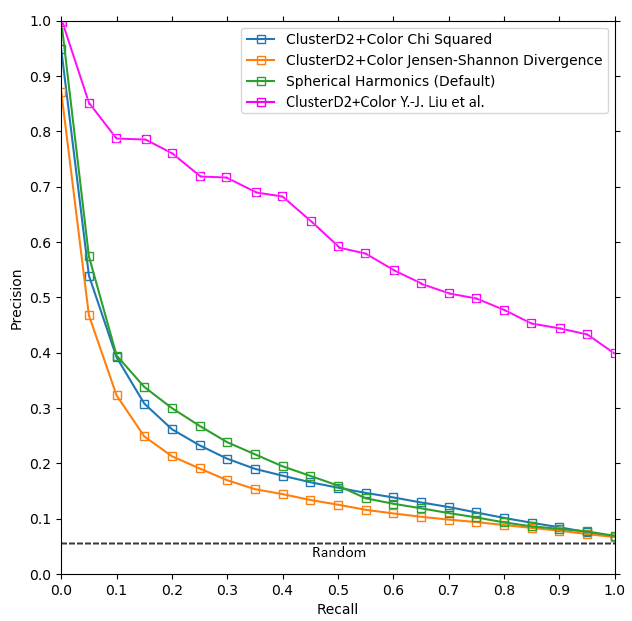
\includegraphics[width=0.5\textwidth]{precision_recall_chisqr_jsd_sh_liu.png}
\caption{Precision/recall plots comparing the performance of Y.-J. Liu et al.'s (pink) and our implementation (blue, orange) of the ClusterD2+Color algorithm using the McGill 3D shape benchmark \cite{mcgill_shape_benchmark} and Cineast's "Spherical Harmonics (Default)" feature module (green). The random scoring baseline is calculated as the average of $\frac{P}{P+N}$ over all classes where $P$ is the number of positives and $N$ the number of negatives.}
\label{fig:precision_recall}
\end{figure}

There are several ways to compare the performance and retrieval quality of different algorithms. One way to do so are precision/recall plots as shown in Fig. \ref{fig:precision_recall}. The larger the area under the
curve the better the algorithm performs. Our precision/recall plots have been computed in the same way as described by Y.-J. Liu et al. \cite{cluster_d2_color} and also using the same model benchmark dataset.\\
As can be seen in Fig. \ref{fig:precision_recall} our implementation of the ClusterD2+Color algorithm with both the Jensen-Shannon divergence distance metric, which Y.-J. Liu et al. used,
and the $\chi^2$ distance metric perform significantly worse than that of the original authors of the algorithm. This begs the question whether our implementation is faulty. Visual inspection, using our feature
extraction visualization tool, however shows no obvious errors. Both the shape and color feature samples are concentrated where one would expect and the cluster assignments also look sensible. The code that generates
the histogram feature vector from the clustered samples is simple and short so we deem it unlikely that it contains any errors.\\
One possible explanation could be the many parameters of the algorithm that can be tweaked. Several of these parameters were not specified by Y.-J. Liu et al. and thus had to be chosen and adjusted by us empirically
and may not be optimal.\\
On the other hand our ClusterD2+Color implementation performs similarly to Cineast's "Spherical Harmonics (Default)" feature module, whereas Y.-J. Liu et al.'s is suprisingly vastly better.
So perhaps the discrepancy between our and Y.-J. Liu et al.'s results could be caused by a difference in the McGill 3D shape benchmark model dataset \cite{mcgill_shape_benchmark} or in the way the precision/recall plots are computed. Finally, there's also the possibility that the result in \cite{cluster_d2_color} is incorrect.

\subsection{Voxelizer Performance}

\begin{figure}
\centering
\captionsetup{width=0.8\textwidth}
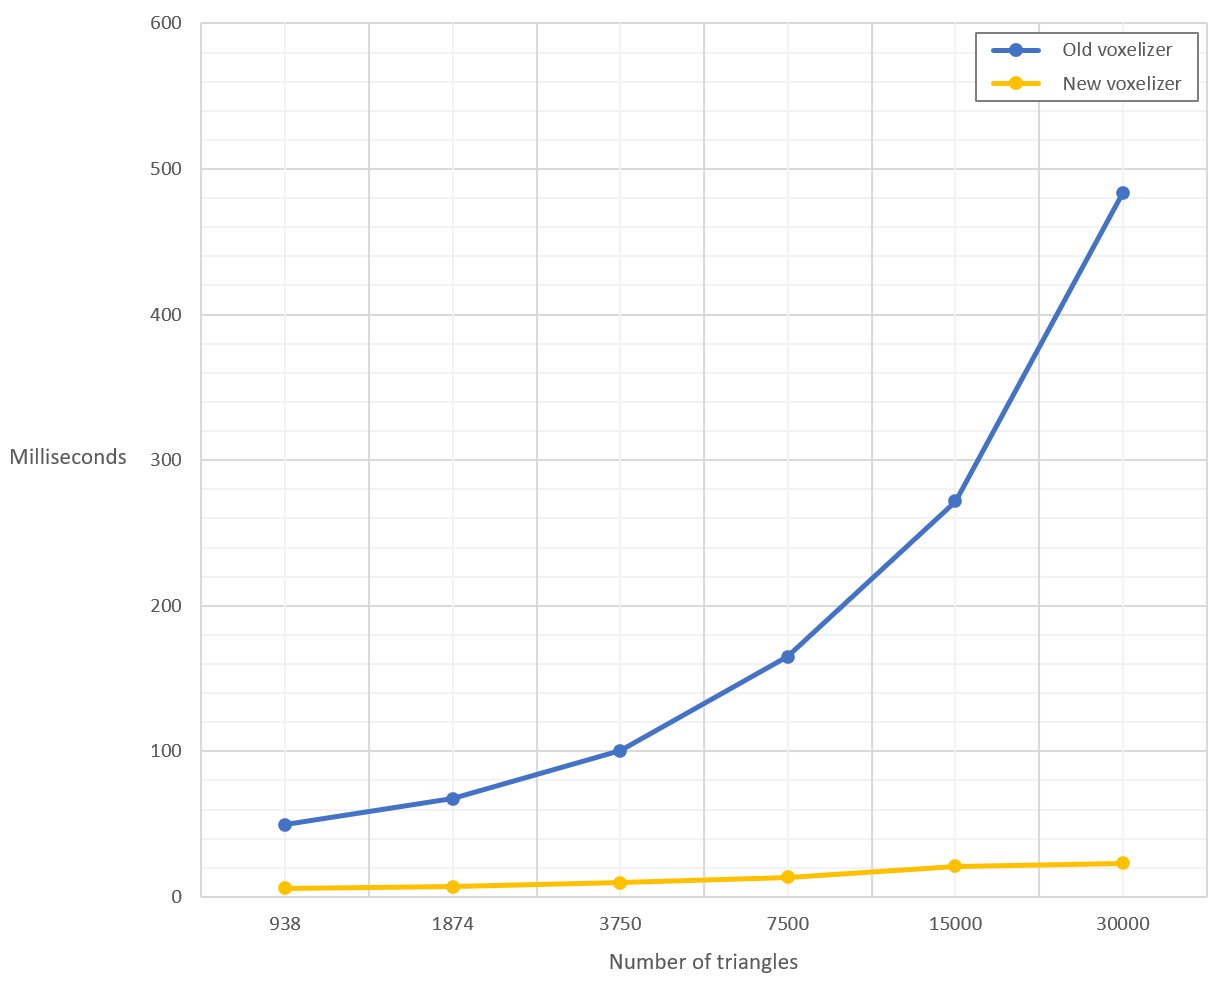
\includegraphics[width=0.5\textwidth]{voxelizer_timings.png}
\caption{Performance comparison between the old and new voxelizer implementation by means of the \cite{stanford_scan_repo} Stanford Armadillo mesh with varying levels of detail. All models were voxelized into a 64x64x64 voxel grid.}
\label{fig:voxelizer_timings}
\end{figure}

The voxel grid resolution was greatly limited in the voxelizer of the precursor prototype, mentioned in Section \ref{sec:approach}, due to lack of performance. For this thesis the voxelizer was rewritten to make better use of Unity's Job System\footnote{\url{https://docs.unity3d.com/2018.3/Documentation/Manual/JobSystem.html}} and to scale better with large meshes using Alg. \ref{alg:assign_triangles} from Section \ref{sec:voxelizer}. From Fig. \ref{fig:voxelizer_timings} it becomes evident that the new voxelizer implementation indeed scales much better with an increasing number of triangles in terms of time taken and is also faster overall due to its better usage of the CPU's eight cores that it was run on.

\section{User Evaluation}

Our application was also tested and evaluated in the form of a user evaluation with the goal of collecting feedback and finding out whether our application is intuitive for new users. This section explains the structure of the user evaluation and its results.

\subsection{Structure}

The user evaluation consists of 11 tasks, grouped into three categories, that the participant should complete within a certain time limit. The first category with two tasks is about the user's background with virtual reality and 3D sculpting applications. The next category with six tasks concerns the usability of the sculpting feature. The remaining three tasks are about the similarity search feature.\\
Before any of the tasks the user was introduced to the topic and was handed the questionnaire to gain an understanding of the user evaluation's structure.\\
The tasks are intended to start out simple and then increase in complexity.\\
The first hands-on task is for the user to read the controller hints, as depicted in Fig. \ref{fig:controller_hints}, to get familiar with the control scheme. During the first few runs it was decided that the user may also try out the controls during this first task.\\
Instead of having to take off the VR headset after every task, the tasks were read to the participant by the user evaluation supervisor and the questionnaire was filled out after all tasks had been completed.\\
Our questionnaire uses a five-point Likert scale, which is the most common approach to capturing data for surveys. These scales offer two or more choices, where each end of the scale corresponds to opposing sentiments or ratings.\\
The complete questionnaire can be found in the Appendix.

\subsection{Sample Size}

In total our user evaluation had 14 participants. Nine of which claim to be moderately or better experienced with virtual reality. Three participants claim to be moderately or better experienced with 3D sculpting applications.\\
This sample size is not large or diverse enough to produce a statistically significant result, however it still allowed us to collect valuable feedback and identify shortcomings in the user interface design or tools of our VR sculpting application.

\subsection{Results Overview}

\begin{figure}
\centering
\captionsetup{width=0.8\textwidth}
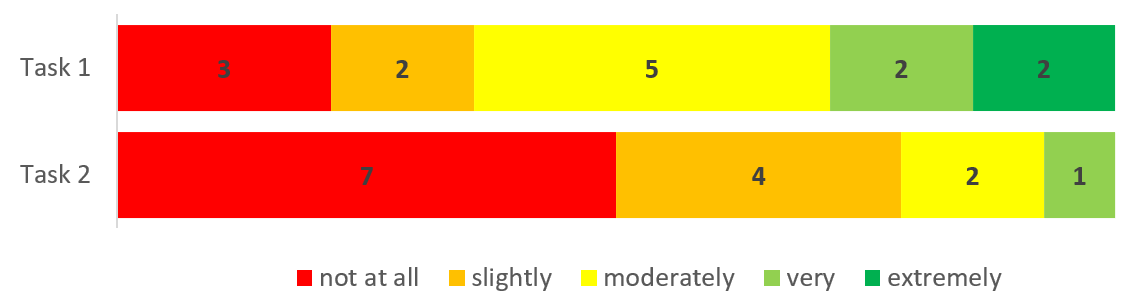
\includegraphics[width=0.5\textwidth]{user_evaluation_tasks_1_2.png}
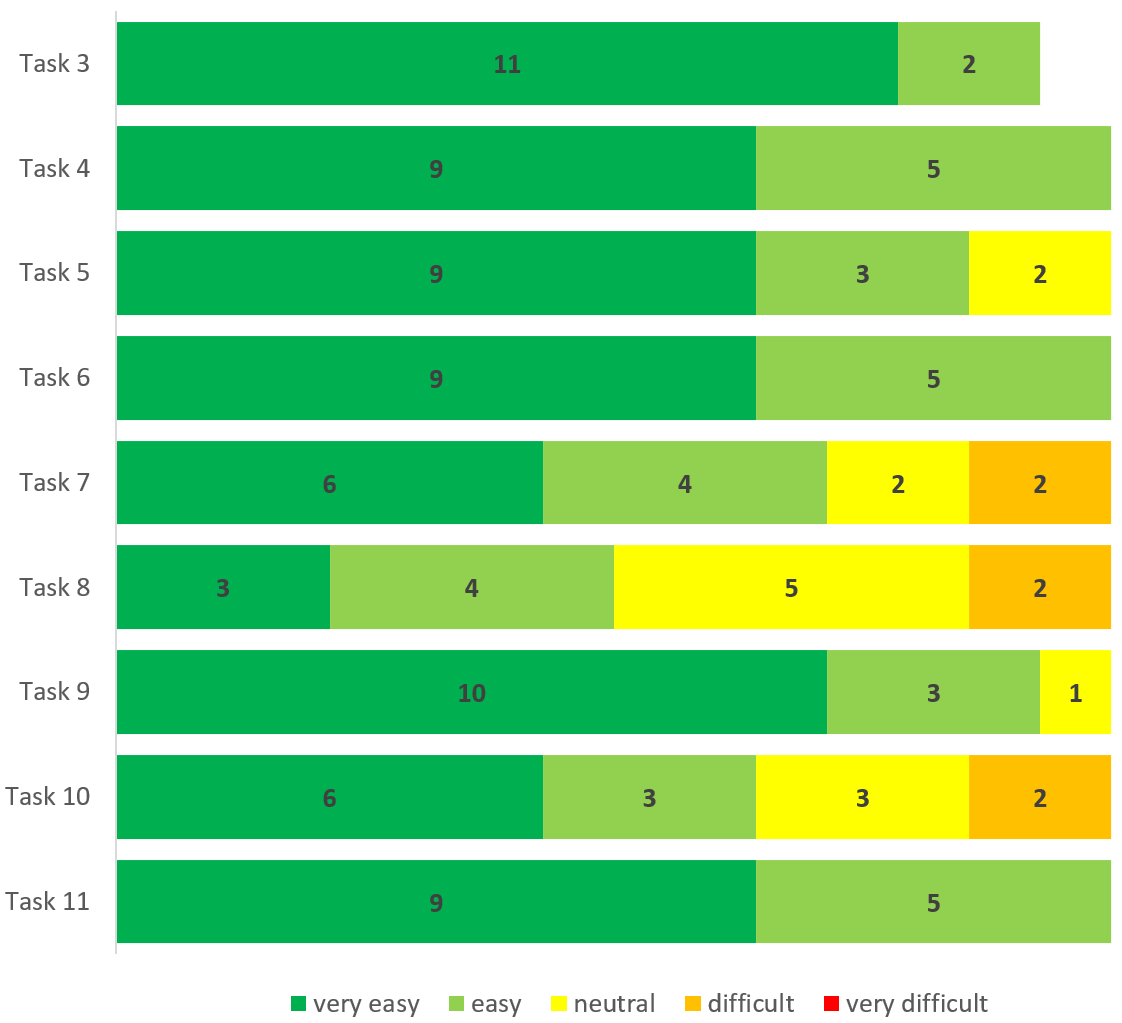
\includegraphics[width=0.5\textwidth]{user_evaluation_tasks_3_11.png}
\caption{The distribution of ratings for each task of the user evaluation.}
\label{fig:user_evaluation_ratings}
\end{figure}

Deducing from the ratings listed in Fig. \ref{fig:user_evaluation_ratings} and the feedback in Section \ref{sec:feedback} the application was perceived as positive and easy to use for the most part. However, it needs to be noted that many participants had stated, while trying out the application, that it became intuitive once they had figured out the controls to use the tools. This means that it may be a bit less intuitive than the final ratings portray.

\begin{table}[ht]
\captionsetup{width=0.8\textwidth}
\caption{Average rating of each task rounded to three significant digits. Same scales apply as in Fig. \ref{fig:user_evaluation_ratings}.}
\centering
\footnotesize
\begin{tabular}{||c c c c c c c c c c c||}
	\hline
	Task 1 & Task 2 & Task 3 & Task 4 & Task 5 & Task 6 & Task 7 & Task 8 & Task 9 & Task 10 & Task 11\\ [0.5ex] \hhline{||===========||}
	2.86 & 1.79 & 1.15 & 1.36 & 1.5 & 1.36 & 2 & 2.43 & 1.36 & 2.07 & 1.36\\ 
	\hline
\end{tabular}
\label{table:user_evaluation_averages}
\end{table}

According to Table \ref{table:user_evaluation_averages} none of the practical tasks, 3 through 11, were rated 3 or higher on average. This means that, on average, they were all considered very easy, easy or somewhere between easy and neutral. Task 8, which had users create a custom brush shape using the custom brush editor, was clearly considered the most difficult, which can be attributed to its partially unintuitive user interface and performance issues. Task 10, which had the users voxelize a query result, was also considered a difficult task because the grip buttons of the VR controllers are difficult to find and uncomfortable use. Lastly task 7, which was about changing the texture/material of the brush, was also rated comparatively difficult because the participants had difficulty finding the correct button on the user interface.

\subsection{Feedback}
\label{sec:feedback}

Tasks one and two, which ask how much experience the participants has with virtual reality and 3D sculpting applications, will be skipped here since there is no feedback from those.\\
Some of the comments have been edited in square brackets by us to clarify the intent of the comment to the reader.\\
P1 through P14 refer to the anonymized user evaluation participants.

\subparagraph{Task 3} \hfill \\
Description: "Read the controller hints to become familiar with VR and the control scheme. Disable the controller hints once you're ready. Please note that you can activate these hints
again at any time if necessary."\\
Feedback:
\begin{itemize} \setlength\itemsep{-0.5em}
	\item[--] P1: Put the arrows for the side buttons [of the trackpad] at the exact position. Picture for direction field [trackpad] (for easier left/right/top/bottom) if possible
	\item[--] P2: The hints on the buttons were tiny bit large where required me to take them away to read them, maybe smaller font size?
	\item[--] P4: For the buttons at the side [grip buttons], it is not immediately clear, that they belong to the voxelize interaction
	\item[--] P5: Appears very cluttered at first
	\item[--] P13: It was sometimes difficult to get the VPad [trackpad] to accept the direction I wanted (e.g. it showed query settings [menu] instead of brush [menu])
\end{itemize}
One participant did not rate this task because they found it unclear what to rate.\\
As depicted in Fig. \ref{fig:controller_hints} the controller hints for the trackpad all point to the center of the trackpad. At this point in time the Unity SteamVR plugin does not provide a way to get them to point to the sides of the trackpad, but this problem could be fixed in the future since the source code of the scripts responsible for said feature can be fully edited.

\subparagraph{Task 4} \hfill \\
Description: "Select the sphere brush and place it the world to create a shape or simple sculpture using the 'Add' mode."\\
Feedback:
\begin{itemize} \setlength\itemsep{-0.5em}
	\item[--] P2: Once realizing the selection method, it's easy to continue \& apply
	\item[--] P9: Rethink menu titles/labels
	\item[--] P11: It's confusing the first time and gets very intuitive after the 5th time using
	\item[--] P13: Well done! Feature request: point to point fill (e.g. for straight legs)
\end{itemize}

\subparagraph{Task 5} \hfill \\
Description: "Select a brush and create a shape, then select another brush and remove a piece of your sculpture with it using the 'Remove' mode."\\
Feedback:
\begin{enumerate} \setlength\itemsep{-0.5em}
	\item[--] P2: The only difficulty of this task is the trackpad sensitivity which activated different menues [than the one intended].
	\item[--] P9: Rethink menu titles/labels
	\item[--] P13: Well done, this is very intuitive. Request: "Smooth surface" [tool or brush]
\end{enumerate}

\subparagraph{Task 6} \hfill \\
Description: "Select a brush and create a shape, then pick another colour and colour a piece of your sculpture using the 'Replace' mode."\\
Feedback:
\begin{enumerate} \setlength\itemsep{-0.5em}
	\item[--] P2: The saturation selection is not the most intuitive color selection. It's better you have saturation on a value before [the participant probably meant that the default value should be 1 instead of 0]
	\item[--] P9: Rethink menu titles/labels
	\item[--] P12: Replace makes sense when considering voxels, but some people may not realize this can be used to color
	\item[--] P13: Request: Define groups [on the sculpture] and then a "colour entire group" option (e.g. all four legs of a stool)
	\item[--] P14: Use other word than replace
\end{enumerate}
It was observed that a few users had trouble selecting a color because the saturation value is by default at 0, hence without changing that value the color of the preview square does not change at all. An improvement for this was implemented after the use evaluation. Now, when the saturation value is close to 0 and the user changes the hue, the saturation value is automatically set to 1.

\subparagraph{Task 7} \hfill \\
Description: "Select a brush and create a shape, then pick another material (i.e. texture) and change the material of a piece of your sculpture using the 'Replace' mode."\\
Feedback:
\begin{enumerate} \setlength\itemsep{-0.5em}
	\item[--] P1: I thought I have to click the button above/below[?] the texture field [the participant probably means the "Pick" button]
	\item[--] P2: I would suggest there is a different square for color \& texture. Took me a few seconds to realize I need to click on the color square.
	\item[--] P5: Easy if you know how. However, the texture selection is somehow hidden.
	\item[--] P9: Rethink menu titles/labels
	\item[--] P10: Could use a label for texture
	\item[--] P11: Textures are too hidden
	\item[--] P13: Bug/inconvenient: it remembers the color selected $\rightarrow$ unexpected color of material + unclear where to select material.
	\item[--] P14: Difficult to find
\end{enumerate}
It is evident from the comments and ratings that the texture/material selection button was difficult to find for many users. One reason for this is that the default texture is a marble texture that is almost entirely white and thus it is easily missed that the color/texture preview square also shows a texture. This problem was addressed by labeling the color/texture preview square like a regular button in a revision after the user evaluation took palce.

\subparagraph{Task 8} \hfill \\
Description: "Create your own brush (with at least two primitives) using the custom brush editor and then use your own brush to create a shape."\\
Feedback:
\begin{enumerate} \setlength\itemsep{-0.5em}
	\item[--] P1: More difficult to handle than the previous tasks
	\item[--] P2: The middle point (white dot) [center of custom brush] is not very visible. Maybe limiting the space the brush needs to be made in [that was already the case, but probably too large since the participant did not notice], or centeralizing [centering] the shape afterwards would be more intuitive.
	\item[--] P4: It is not very clear how you switch between different components of the texture [participant probably meant brush instead of texture]
	\item[--] P5: That part of the UI is not very intuitive and involves a lot of buttons. Maybe implement as a dedicated "mode".
	\item[--] P11: Kind of hidden
	\item[--] P13: Not that intuitive. Improvements in: snapping to center, rotate [to] fixed value etc... $\rightarrow$ tried to get a triangle shape and that's hard.
\end{enumerate}
The ratings of this task were quite scattered. This is probably the case because some participants tried to make a simple shape and succeeded, whereas others had a more complex shape in mind and then failed due to the unintuitive or lacking
tools of the custom brush editor. These results show that there is still a lot of work required in order to turn this feature into something usable. Another major issue was also the performance drops while using the custom brush editor.

\subparagraph{Task 9} \hfill \\
Description: "Select a brush and create a shape, then use the query menu to run a similarity search."\\
Feedback:
\begin{enumerate} \setlength\itemsep{-0.5em}
	\item[--] P2: Except the framerate drop [when loading in the query results to be displayed] which feels like a VR earthquake it's very easy.
	\item[--] P5: Querying takes a long time.
\end{enumerate}
This task was generally perceived as simple. Several participants noted that the query seems to take a long time. Furthermore for some participants there was a significant framerate drop while the query results were being loaded in. This is definitely something to be improved in the future.

\subparagraph{Task 10} \hfill \\
Description: "Select a brush and create a shape, then use the query menu to run a similarity search. After that, pick one of the results and voxelize it into the world."\\
Feedback:
\begin{enumerate} \setlength\itemsep{-0.5em}
	\item[--] P2: Button nearly impossible to find. I recommend against using the side buttons for such important interactions
	\item[--] P4: Buttons are chosen suboptimally
	\item[--] P5: Grip feels very uncomfortable to me.
	\item[--] P11: It's hard to figure out that you have to grab the item from very near, when sculptures can be grabbed from farther away
\end{enumerate}
Nearly all participants had trouble finding the correct button on the left VR controller. These grip buttons are intended to be pressed by squeezing ones hand or by pressing them with the pinky finger. However, unless one already knows these buttons they're very difficult to find since they don't feel or look like buttons. A solution for this is proposed in Section \ref{sec:future_work}.

\subparagraph{Task 11} \hfill \\
Description: "Select a brush and create a shape, then use the query menu to run a similarity search. After that, pick one of the results and voxelize it. Using a brush, remove a piece of it and then run a similarity search for the modified sculpture."\\
Feedback:
\begin{enumerate} \setlength\itemsep{-0.5em}
	\item[--] P1: Only voxelize was difficult
\end{enumerate}

\subparagraph{General Feedback} \hfill \\
Description: "If you have any additional remarks or suggestions for improvements please write them down here."\\
Feedback:
\begin{enumerate} \setlength\itemsep{-0.5em}
	\item[--] P1: I needed some time to understand the program but then it was relatively easy to use. A visual info about the current mode (add/remove/etc.) would be helpful (adapt color of brush?)
	\item[--] P2: It's a very well done demo, quite entertaining \& interesting. The only drawback of using complex \& memory consuming applications in VR is the very visible \& felt framerate drop which affect the experience. Other than that, the implementation is very smooth. Well done!
	\item[--] P4: Sculpting in general felt easy and intuitive. The evaluation might have benefited from specifying which object the user should sculpt. Good job, impressive result!
	\item[--] P5: Very cool tool! More results would be nice. Sometimes performance drops considerably.
	\item[--] P6: It's a very good project. It would be nice to add some physics and [user created] animations to the model.
	\item[--] P8: The assignment of the functions to the buttons can be improved. Allow the modelling of a second sculpture while the first one is queried. Add more functions which help modelling, similar to the line functionality. (that could also draw for you once you have aligned the line).
	\item[--] P9: Change brush width, height, depth [of regular brushes, not custom brushes]. Works well and is quite easy to understand. Fun to use!
	\item[--] P10: Thought it was excellent. Easy to use, the [controller] hints were incredibly useful and can definitely see the potential.
	\item[--] P11: The whole experience felt surprisingly real and immersive. "Mouse clicks" [from the VR controller pointer] are a thing I had to get used to.
	\item[--] P13: Great demo/prototype! Apparently, there are some minor differences during feature extraction, as the stool was not found using it [voxelized stool] as query, but returned almost always as if something other was queried for. Request: Add larger "brushes" for weights $\rightarrow$ prioritise the shape of a certain part... [the participant probably means that there should be a tool to select certain parts of the sculpture such that brushes only (or mostly) affect those selected parts]
	\item[--] P14: Better manual to know where the textures are. Voxelizing is a little tricky.
\end{enumerate}

The suggestion of P1, changing the color of the brush depending on the brush mode, was implemented after the user evaluation. In the union mode the brushes remain the default blue color, in remove mode they become red and in replace mode green. Overall a lot of useful feedback was provided. Several interesting ideas have been brought up and are mentioned later in Section \ref{sec:future_work}.